A subdivision surface is the limit surface resulted from the
application of a subdivision algorithm to a control polyhedron.
Subdivision algorithms recursively \emph{refine} (subdivide) the
control polyhedron and \emph{modify} (smooth) the geometry according
to the stencils of the source mesh.  Subdivisions consist of two
meta-steps that most geometry processing algorithms have: the
\emph{connectivity operation} and the
\emph{geometry operation}. In this paper, we use subdivision
as the template of the geometry processing algorithms because it
connectivity operations are more complex than most other
algorithms. Some other simple algorithms, e.g.\ displacement map, the
connectivity operation is a null operation. In other words, the source
and the target mesh have the same connectivity.  Further details on
subdivisions can be found at \cite{siggraph1998notes}.

% pierre: isnt it better to take Sig 2000 course notes instead?

We characterize subdivision algorithms as the combination of the
\emph{refinement operator} and the \emph{modification operator(s)}. 
The refinement operator edits the connectivity and create a uniformly
refined mesh from the source polyhedron.  Refinement operators are
classified according to the connectivity pattern and the topology
correspondence.  Figure \ref{RefSchemes} shows four major refinements
employed in subdivision algorithms, which include Catmull-Clark
subdivision (PQQ) \cite{cc}, Loop subdivision (PTQ) \cite{loop},
Doo-Sabin subdivision (DQQ) \cite{ds} and $\sqrt{3}$ subdivision
\cite{sqrt3}. Subdivisions, such as Quad-Triangle subdivision (PQQ +
PTQ) \cite{qts,l-pg-03}, may employ a hybrid refinement that combines
two different refinements.

\begin{figure}
  \centering
  \psfrag{PQQ}[]{\scriptsize PQQ} 
  \psfrag{PTQ}[]{\scriptsize PTQ}
  \psfrag{DQQ}[]{\scriptsize DQQ} 
  \psfrag{Sqrt3}[]{\scriptsize $\sqrt{3}$} 
  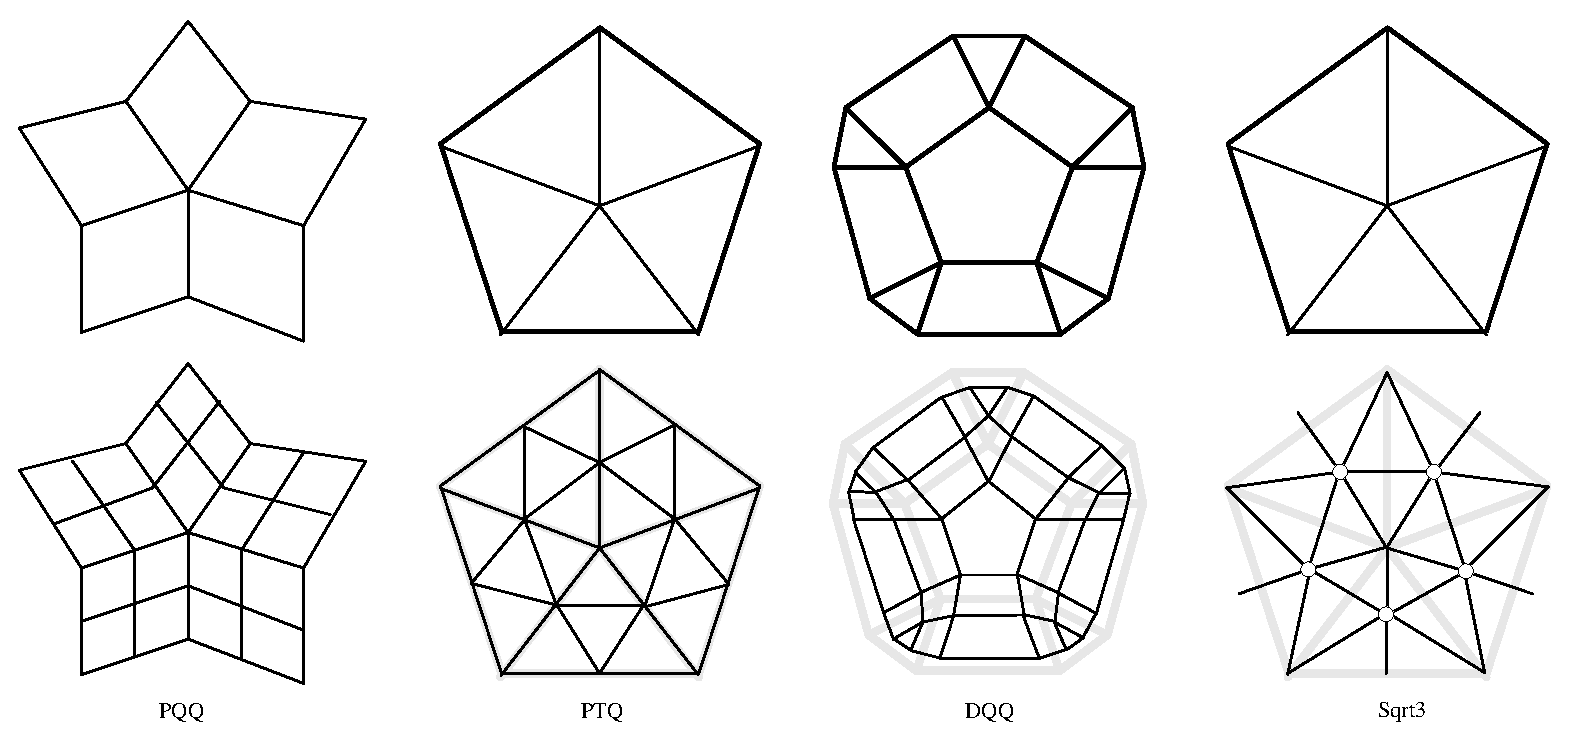
\epsfig{file=figs/RefSchemes.eps, width=7cm}
  \caption{Refinement operators: 
    primal quadrilateral quadrisection (PQQ),
    primal triangle quadrisection (PTQ),
    dual quadrilateral quadrisection (DQQ) and
    $\sqrt{3}$ triangulation.}
  \label{fig:RefSchemes}
\end{figure}

The modification operator collects the stencil (submesh) of the source
polyhedron and applies a mask (weighted map) on the stencil to
generate the corresponding vertex of the target (refined)
polyhedron. Figure \ref{fig:RefMap} demonstrates the examples of the
correspondence between a stencil and its smoothed
vertices. Subdivisions usually have several modification operators
associated with different different types of stencils (Figure
\ref{fig:RefMap} (a-c)).  The modification operators iterate on all
entities of the target mesh.

\begin{figure}
  \centering
  \psfrag{A}[]{(a)}
  \psfrag{B}[]{(b)}
  \psfrag{C}[]{(c)}
  \psfrag{D}[]{(d)}
  \epsfig{file=figs/RefMap.eps, width=7cm}
  \caption{The correspondence of the stencil and the 
           target vertex in the Catmull-Clark subdivision (a-c)
	   and Doo-Sabin subdivision (d). Catmull-Clark
	   subdivision has three stencils: facet-stencil (a), 
	   edge-stencil (b) and vertex-stencil (c).}
  \label{fig:RefMap}
\end{figure}

In the following two sections, we demonstrate the implementation of
the subdivisions based on the \cgalpoly.  We introduce two
non-polymorphism designs of the subdivisions.  To support the
refinement operators, one applies the atomic connectivity operators
and the other uses the modifier of the \cgalpoly.  The modification
operations are statically wired in the refinement operator. The
polymorphism design is shown latter in section \ref{sect:} where
modification operators are abstracted from the refinement.


% connectivity ops: specific polyhedron algorithms (sqrt3 subdivisions) 
\subsection{$\sqrt{3}$-Subdivision using Euler Operators}
\input sqrt3

% inc builder: specific polyhedron algorithms (qt subdivisions) 
\subsection{Quad-triangle Subdivision using modifier}
\input qt

% templated rules: a generic framework for subdivisions 
\subsection{Generic Subdivisions}
%\label{sec:subtempl}
\input subtempl